% Release 1: Core Architecture & Communities
\chapter{Release 1: Core Architecture \& Communities}

\section*{High-Level Planning}
The development of this Discord Clone is organized into two primary releases, following the Agile SCRUM methodology. This strategic division ensures that foundational features are established before complex real-time functionalities are introduced. 
\begin{itemize}
    \item \textbf{Release 1: Core Architecture \& Communities} encompasses Sprint 1 (Authentication) and Sprint 2 (Servers/Roles). This release focuses on secure user registration, identity management, and the creation of isolated collaboration spaces.
    \item \textbf{Release 2: Real-Time Communication} encompasses Sprint 3 (Text Chat) and Sprint 4 (Voice Channels). This release introduces live WebSocket-based messaging and WebRTC-based peer-to-peer voice communications.
\end{itemize}

\section{Sprint 1: Authentication}

\subsection{Sprint Overview}
The primary objective of Sprint 1 is to establish a secure and reliable authentication system. The sprint backlog is detailed in Table~\ref{tab:sprint1_backlog}.

\begin{table}[H]
    \centering
    \begin{tabular}{|c|p{10cm}|c|}
        \hline
        \textbf{ID} & \textbf{Description} & \textbf{Priority} \\
        \hline
        S1-01 & As a new user, I want to register an account, So that I can access the platform. & P0 \\
        \hline
        S1-02 & As a registered user, I want to log in with email/password, So that I can access my account. & P0 \\
        \hline
        S1-03 & As a logged-in user, I want to log out, So that my session is securely closed. & P1 \\
        \hline
        S1-04 & As a logged-in user, I want to view/edit my display name, So that I can personalize my profile. & P1 \\
        \hline
    \end{tabular}
    \caption{Sprint 1 Backlog: Authentication}
    \label{tab:sprint1_backlog}
\end{table}

\subsection{Analysis and Design}
During this initial sprint, the system architecture lays the foundation for user management and security. 

\begin{figure}[H]
    \centering
    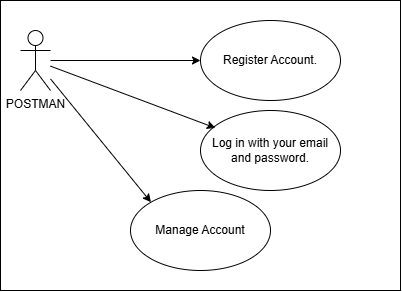
\includegraphics[width=0.7\textwidth]{use_case_sprint1.png}
    \caption{Use Case Diagram for Sprint 1 (Authentication \& Profile)}
    \label{fig:use_case_sprint1}
\end{figure}

The Use Case Diagram above illustrates the base actions available to an unauthenticated and authenticated user. These fundamental use cases, such as "Register" and "Log In", will act as prerequisites for all subsequent interactions in future sprints.

\begin{figure}[h!]
    \centering
    \rule{0.8\textwidth}{5cm} % Placeholder box
    \caption{[INSERT SPECIFIC DIAGRAM/SCREENSHOT HERE: Class Diagram for Sprint 1]}
    \label{fig:sprint1_class}
\end{figure}

The initial database model consists of the core \texttt{User} entity, which stores credentials and profile metadata. This class forms the root of the database relationships, to which servers, channels, and messages will be linked in subsequent iterations.

\begin{table}[h!]
    \centering
    \begin{tabular}{|p{4cm}|p{10cm}|}
        \hline
        \textbf{Use Case} & \textbf{Log In} \\
        \hline
        \textbf{Primary Actor} & Registered User \\
        \hline
        \textbf{Main Success Scenario} & 1. User provides email and password. \newline 2. System validates credentials. \newline 3. System issues an authentication token. \newline 4. User is redirected to the dashboard. \\
        \hline
    \end{tabular}
    \caption{Main Use Case Description: Log In}
    \label{tab:sprint1_uc_desc}
\end{table}

\begin{figure}[h!]
    \centering
    \rule{0.8\textwidth}{5cm} % Placeholder box
    \caption{[INSERT SPECIFIC DIAGRAM/SCREENSHOT HERE: Sequence Diagram for Authentication Flow]}
    \label{fig:sprint1_sequence}
\end{figure}

\subsection{Sprint Review}
Sprint 1 successfully delivered a functional authentication flow. The registration and login endpoints were integrated with the frontend interface, allowing users to securely access the platform.

\begin{figure}[h!]
    \centering
    \rule{0.8\textwidth}{5cm} % Placeholder box
    \caption{[INSERT SPECIFIC DIAGRAM/SCREENSHOT HERE: Screenshot of Login/Register UI]}
    \label{fig:sprint1_ui}
\end{figure}

As illustrated in Figure \ref{fig:sprint1_ui}, the user inputs their credentials into the registration form. Upon successful submission, a secure session is established, and the user is navigated to their profile where they can view and edit their display name.

\subsection{Sprint Retrospective}
The retrospective for Sprint 1 highlights the achievements and the technical hurdles encountered during the implementation of the security layer.

\begin{table}[h!]
    \centering
    \begin{tabular}{|p{7cm}|p{7cm}|}
        \hline
        \textbf{Successes} & \textbf{Missing Elements / Challenges} \\
        \hline
        - Secure password hashing implemented. \newline - JWT-based session management operational. \newline - Profile updating functional. & - Setting up secure HTTP-only cookies across CORS boundaries was challenging. \newline - Email verification is currently missing and deferred to a later release. \\
        \hline
    \end{tabular}
    \caption{Sprint 1 Retrospective}
    \label{tab:sprint1_retro}
\end{table}


\section{Sprint 2: Servers}

\subsection{Sprint Overview}
With authentication in place, Sprint 2 focuses on creating isolated communities, termed "Servers", along with their respective channels and roles.

\begin{table}[h!]
    \centering
    \begin{tabular}{|c|p{10cm}|c|}
        \hline
        \textbf{ID} & \textbf{Description} & \textbf{Priority} \\
        \hline
        S2-01 & As a user, I want to create a new server, So that I can build a community. & P0 \\
        \hline
        S2-02 & As a server owner, I want to generate an invite link, So that others can join. & P0 \\
        \hline
        S2-03 & As a user, I want to join a server using an invite link, So that I can participate. & P0 \\
        \hline
        S2-04 & As a server owner, I want to create text/voice channels, So that I can organize discussions. & P1 \\
        \hline
        S2-05 & As a server owner, I want to create/assign roles, So that I can manage permissions. & P1 \\
        \hline
    \end{tabular}
    \caption{Sprint 2 Backlog: Servers}
    \label{tab:sprint2_backlog}
\end{table}

\subsection{Analysis and Design}
Building upon the authenticated user context from Sprint 1, this sprint introduces community management architectures.

\begin{figure}[h!]
    \centering
    \rule{0.8\textwidth}{5cm} % Placeholder box
    \caption{[INSERT SPECIFIC DIAGRAM/SCREENSHOT HERE: Use Case Diagram for Sprint 2]}
    \label{fig:sprint2_usecase}
\end{figure}

As shown above, the new use cases such as "Create a Server" and "Join a Server" MUST \texttt{<<include>>} the "Log In" use case from Sprint 1. The system enforces that only authenticated users can execute these community actions.

\begin{figure}[h!]
    \centering
    \rule{0.8\textwidth}{5cm} % Placeholder box
    \caption{[INSERT SPECIFIC DIAGRAM/SCREENSHOT HERE: Class Diagram for Sprint 2]}
    \label{fig:sprint2_class}
\end{figure}

The database model grows significantly in this sprint. The \texttt{Server}, \texttt{Channel}, and \texttt{Role} classes are introduced. A many-to-many relationship (often resolved via a \texttt{ServerMember} junction class) maps the \texttt{User} class from Sprint 1 to the new \texttt{Server} class, dictating community memberships.

\begin{table}[h!]
    \centering
    \begin{tabular}{|p{4cm}|p{10cm}|}
        \hline
        \textbf{Use Case} & \textbf{Join a Server} \\
        \hline
        \textbf{Primary Actor} & Authenticated User \\
        \hline
        \textbf{Main Success Scenario} & 1. User clicks an invite link. \newline 2. System validates the invite token. \newline 3. User is added to the server's member list. \newline 4. User views the server's default channels. \\
        \hline
    \end{tabular}
    \caption{Main Use Case Description: Join a Server}
    \label{tab:sprint2_uc_desc}
\end{table}

\begin{figure}[h!]
    \centering
    \rule{0.8\textwidth}{5cm} % Placeholder box
    \caption{[INSERT SPECIFIC DIAGRAM/SCREENSHOT HERE: Activity Diagram for Creating a Server]}
    \label{fig:sprint2_activity}
\end{figure}

\subsection{Sprint Review}
Sprint 2 successfully established the core community framework. Users can now create servers, generate invite links, and organize their communities with text and voice channels.

\begin{figure}[h!]
    \centering
    \rule{0.8\textwidth}{5cm} % Placeholder box
    \caption{[INSERT SPECIFIC DIAGRAM/SCREENSHOT HERE: Screenshot of Server Dashboard and Invite UI]}
    \label{fig:sprint2_ui}
\end{figure}

As illustrated in Figure \ref{fig:sprint2_ui}, the user navigates the sidebar to create a server. Upon creation, the owner is presented with the server dashboard where they can manage roles and generate unique invite links to distribute to other users.

\subsection{Sprint Retrospective}
The introduction of relational community data presented new operational challenges.

\begin{table}[h!]
    \centering
    \begin{tabular}{|p{7cm}|p{7cm}|}
        \hline
        \textbf{Successes} & \textbf{Missing Elements / Challenges} \\
        \hline
        - Server creation and member association works seamlessly. \newline - Dynamic invite link generation implemented. \newline - Channel and role structures successfully persisted. & - Managing cascading deletes (e.g., deleting a server must delete all associated channels and roles) required complex database constraints. \newline - Advanced role permission inheritance is incomplete. \\
        \hline
    \end{tabular}
    \caption{Sprint 2 Retrospective}
    \label{tab:sprint2_retro}
\end{table}


% Release 2: Real-Time Communication
\chapter{Release 2: Real-Time Communication}

\section{Sprint 3: Text Chat}

\subsection{Sprint Overview}
Sprint 3 initiates Release 2 by introducing real-time text messaging capabilities within the server channels created in Sprint 2.

\begin{table}[h!]
    \centering
    \begin{tabular}{|c|p{10cm}|c|}
        \hline
        \textbf{ID} & \textbf{Description} & \textbf{Priority} \\
        \hline
        S3-01 & As a member, I want to send a message in a text channel instantly, So that I can chat with others. & P0 \\
        \hline
        S3-02 & As a member, I want to see recent messages chronologically, So that I can follow the conversation. & P1 \\
        \hline
        S3-03 & As a member, I want to see online/offline status of others, So that I know who is active. & P1 \\
        \hline
        S3-04 & As a member, I want to mention others using @username, So that I can notify them directly. & P2 \\
        \hline
    \end{tabular}
    \caption{Sprint 3 Backlog: Text Chat}
    \label{tab:sprint3_backlog}
\end{table}

\subsection{Analysis and Design}
This sprint shifts the architectural focus toward real-time bi-directional communication using WebSockets.

\begin{figure}[h!]
    \centering
    \rule{0.8\textwidth}{5cm} % Placeholder box
    \caption{[INSERT SPECIFIC DIAGRAM/SCREENSHOT HERE: Use Case Diagram for Sprint 3]}
    \label{fig:sprint3_usecase}
\end{figure}

The text messaging use cases inherently rely on the community structure. "Send a Message" extends the user's capabilities inside a specific text channel, requiring validation that the user is an active member of the server (a constraint established in Sprint 2).

\begin{figure}[h!]
    \centering
    \rule{0.8\textwidth}{5cm} % Placeholder box
    \caption{[INSERT SPECIFIC DIAGRAM/SCREENSHOT HERE: Class Diagram for Sprint 3]}
    \label{fig:sprint3_class}
\end{figure}

The database model is expanded with the \texttt{Message} class. This new entity maps directly to the \texttt{Channel} class from Sprint 2 (indicating where the message was sent) and the \texttt{User} class from Sprint 1 (indicating the author). This relational chaining creates a comprehensive history of interactions.

\begin{table}[h!]
    \centering
    \begin{tabular}{|p{4cm}|p{10cm}|}
        \hline
        \textbf{Use Case} & \textbf{Send a Message} \\
        \hline
        \textbf{Primary Actor} & Server Member \\
        \hline
        \textbf{Main Success Scenario} & 1. Member types a message and submits. \newline 2. Client emits a WebSocket event. \newline 3. Server persists the message to the database. \newline 4. Server broadcasts the message to all clients in the channel. \\
        \hline
    \end{tabular}
    \caption{Main Use Case Description: Send a Message}
    \label{tab:sprint3_uc_desc}
\end{table}

\begin{figure}[h!]
    \centering
    \rule{0.8\textwidth}{5cm} % Placeholder box
    \caption{[INSERT SPECIFIC DIAGRAM/SCREENSHOT HERE: Sequence Diagram for WebSocket Messaging]}
    \label{fig:sprint3_sequence}
\end{figure}

\subsection{Sprint Review}
The text chat functionality was successfully deployed, enabling instantaneous communication. Users can see messages appear live, view historical messages, and track user presence.

\begin{figure}[h!]
    \centering
    \rule{0.8\textwidth}{5cm} % Placeholder box
    \caption{[INSERT SPECIFIC DIAGRAM/SCREENSHOT HERE: Screenshot of Text Channel Interface]}
    \label{fig:sprint3_ui}
\end{figure}

As illustrated in Figure \ref{fig:sprint3_ui}, the user selects a text channel from the sidebar. The central view populates with chronological messages. Typing in the input box and pressing enter instantly pushes the message to the interface of all connected members via WebSockets.

\subsection{Sprint Retrospective}
Implementing real-time state synchronization introduced significant technical complexities.

\begin{table}[h!]
    \centering
    \begin{tabular}{|p{7cm}|p{7cm}|}
        \hline
        \textbf{Successes} & \textbf{Missing Elements / Challenges} \\
        \hline
        - Real-time WebSocket broadcasting is exceptionally fast. \newline - Message history retrieval works efficiently. \newline - Mentioning users correctly triggers frontend highlights. & - Handling real-time WebSocket state and connection drops required implementing complex reconnection logic. \newline - Synchronizing online/offline presence at scale proved difficult and occasionally desynchronizes. \\
        \hline
    \end{tabular}
    \caption{Sprint 3 Retrospective}
    \label{tab:sprint3_retro}
\end{table}


\section{Sprint 4: Voice}

\subsection{Sprint Overview}
The final sprint introduces the most complex feature: real-time voice communication channels.

\begin{table}[h!]
    \centering
    \begin{tabular}{|c|p{10cm}|c|}
        \hline
        \textbf{ID} & \textbf{Description} & \textbf{Priority} \\
        \hline
        S4-01 & As a member, I want to join a voice channel and talk in real-time, So that I can converse verbally. & P0 \\
        \hline
        S4-02 & As a participant, I want to mute my microphone, So that others cannot hear me. & P1 \\
        \hline
        S4-03 & As a participant, I want to deafen myself, So that I do not hear others. & P1 \\
        \hline
        S4-04 & As a participant, I want to see who is currently speaking, So that I can identify active talkers. & P1 \\
        \hline
    \end{tabular}
    \caption{Sprint 4 Backlog: Voice Channels}
    \label{tab:sprint4_backlog}
\end{table}

\subsection{Analysis and Design}
This sprint builds on the WebSocket signaling infrastructure created in Sprint 3 to establish Peer-to-Peer or SFU (Selective Forwarding Unit) WebRTC connections.

\begin{figure}[h!]
    \centering
    \rule{0.8\textwidth}{5cm} % Placeholder box
    \caption{[INSERT SPECIFIC DIAGRAM/SCREENSHOT HERE: Use Case Diagram for Sprint 4]}
    \label{fig:sprint4_usecase}
\end{figure}

The "Join Voice Channel" use case represents the pinnacle of the application's complexity. It utilizes the community roles (Sprint 2) to authorize entry and the WebSocket connections (Sprint 3) to negotiate the media streams.

\begin{figure}[h!]
    \centering
    \rule{0.8\textwidth}{5cm} % Placeholder box
    \caption{[INSERT SPECIFIC DIAGRAM/SCREENSHOT HERE: Class Diagram for Sprint 4]}
    \label{fig:sprint4_class}
\end{figure}

The database schema experiences minor additions, primarily tracking active voice sessions or specific voice channel settings. However, the architectural growth is predominantly in the client-side state management handling WebRTC \texttt{RTCPeerConnection} objects.

\begin{table}[h!]
    \centering
    \begin{tabular}{|p{4cm}|p{10cm}|}
        \hline
        \textbf{Use Case} & \textbf{Join a Voice Channel} \\
        \hline
        \textbf{Primary Actor} & Server Member \\
        \hline
        \textbf{Main Success Scenario} & 1. User clicks on a voice channel. \newline 2. Client requests microphone permissions. \newline 3. Client exchanges WebRTC SDP offers/answers via WebSockets. \newline 4. P2P media streams are established. \\
        \hline
    \end{tabular}
    \caption{Main Use Case Description: Join a Voice Channel}
    \label{tab:sprint4_uc_desc}
\end{table}

\begin{figure}[h!]
    \centering
    \rule{0.8\textwidth}{5cm} % Placeholder box
    \caption{[INSERT SPECIFIC DIAGRAM/SCREENSHOT HERE: Sequence Diagram for WebRTC Negotiation]}
    \label{fig:sprint4_sequence}
\end{figure}

\subsection{Sprint Review}
Voice channels were successfully integrated. Users can seamlessly join a voice room, transmit audio, and utilize mute/deafen controls while observing active speaker indicators.

\begin{figure}[h!]
    \centering
    \rule{0.8\textwidth}{5cm} % Placeholder box
    \caption{[INSERT SPECIFIC DIAGRAM/SCREENSHOT HERE: Screenshot of Voice Channel UI with Active Speakers]}
    \label{fig:sprint4_ui}
\end{figure}

As illustrated in Figure \ref{fig:sprint4_ui}, clicking on a voice channel instantly connects the user. The interface updates to show user avatars within the channel. When a participant speaks, a green border highlights their avatar, providing immediate visual feedback of the active speaker.

\subsection{Sprint Retrospective}
Integrating WebRTC provided the most significant learning curve of the project.

\begin{table}[H]
    \centering
    \begin{tabular}{|p{7cm}|p{7cm}|}
        \hline
        \textbf{Successes} & \textbf{Missing Elements / Challenges} \\
        \hline
        - WebRTC audio transmission is clear and low-latency. \newline - Hardware controls (mute/deafen) correctly stop media tracks. \newline - Active speaker detection accurately updates the UI. & - Managing WebRTC STUN/TURN servers for clients behind strict NATs was a major networking challenge. \newline - Scaling voice channels beyond a few users degrades performance without a dedicated SFU server, which remains a future optimization. \\
        \hline
    \end{tabular}
    \caption{Sprint 4 Retrospective}
    \label{tab:sprint4_retro}
\end{table}
